% =============================================================
%  EE-559 mini-project paper  (3-page limit, IEEE references)
%  Hate speech detection : text & multimodal
% =============================================================
\documentclass[10pt,a4paper,twocolumn]{article}

\usepackage[utf8]{inputenc}
\usepackage[T1]{fontenc}
\usepackage[english]{babel}
\usepackage[a4paper,margin=1.7cm]{geometry}
\usepackage{lmodern}
\usepackage{microtype}
\usepackage{graphicx}
\usepackage{booktabs}
\usepackage{amsmath,amssymb}
\usepackage{xcolor}
\usepackage{hyperref}
\usepackage{caption}
\usepackage{titlesec}
\usepackage{enumitem}

\hypersetup{colorlinks=true, linkcolor=black, citecolor=blue!50!black, urlcolor=blue!60!black}

% Tighter section spacing
\titlespacing*{\section}{0pt}{1.0ex plus 0.3ex minus .2ex}{0.6ex plus .2ex}
\titlespacing*{\subsection}{0pt}{0.7ex plus 0.2ex minus .1ex}{0.4ex plus .1ex}
\titleformat{\section}{\normalsize\bfseries}{\thesection.}{0.6em}{}
\titleformat{\subsection}{\small\bfseries}{\thesubsection}{0.5em}{}

\setlength{\abovecaptionskip}{2pt}
\setlength{\belowcaptionskip}{1pt}
\setlength{\textfloatsep}{6pt plus 1pt minus 1pt}
\setlength{\intextsep}{6pt plus 1pt minus 1pt}
\setlength{\parskip}{1pt}
\captionsetup{font=small,labelfont=bf,skip=2pt}

\renewcommand{\refname}{\vspace{-1ex}\normalsize References}

% -------- Title block --------
\title{\vspace{-2em}\textbf{Hate Speech Detection: \\[-0.2em]
Text and Multimodal Approaches with a Bias Analysis}\vspace{-1em}}
\author{\normalsize [Author 1] \quad [Author 2] \quad [Author 3] \\[-0.2em]
\small Group [GroupNumber]\vspace{-2em}}
\date{}

\begin{document}
\twocolumn[
\begin{@twocolumnfalse}
\maketitle
\begin{abstract}\small
\noindent We tackle hate speech detection on two benchmarks: (i) HateXplain~\cite{hatexplain}, a 3-class text dataset, and (ii) HarMeme~\cite{harmeme}, a multimodal harmful-meme dataset. On HateXplain we fine-tune HateBERT~\cite{hatebert} with focal loss~\cite{focal} and label-confidence weighting, reaching test macro-F1 $=0.683$. We then quantify a target-group bias gap of $0.22$ macro-F1 across 11 groups and test two correction strategies --- inverse-frequency group weighting and counterfactual lexical augmentation~\cite{liang} --- both of which fail and widen the gap, an instructive negative result aligned with~\cite{davidson,sap}. On HarMeme we compare CLIP+HateBERT~\cite{clip} under frozen, defrost, and cross-attention fusion: partial defrost of the last two encoder layers is best (test AUROC $=0.910$). We additionally report a silent data-loader bug that invalidated eight prior multimodal runs --- a methodological lesson on validating multimodal pipelines.

\smallskip\noindent\textbf{Keywords:} hate speech, multimodal classification, HateBERT, CLIP, fairness analysis.
\end{abstract}
\vspace{0.6em}
\end{@twocolumnfalse}
]

% =============================================================
\section{Introduction}
% =============================================================

Hate speech detection is societally high-stakes but intrinsically ambiguous: the boundary between \emph{offensive} and \emph{hateful} content is fuzzy, and 33\% of HateXplain annotations on the \emph{offensive} class show inter-annotator disagreement~\cite{hatexplain}. We address two questions. \textbf{(Q1)} Can a domain-adapted text encoder cleanly separate hate, normal, and offensive posts, and are the residual errors a modelling or an annotation problem? \textbf{(Q2)} When images are added (memes), does multimodal fusion help, and which fusion regime suits small datasets?

We further investigate a fairness limitation reported in the literature: spurious associations between target-group mentions and the \emph{hate} label~\cite{davidson,sap}. We test two simple mitigation strategies and report both as negative results, characterising their failure mode rather than presenting a misleading improvement.

\textbf{Contributions.} (1)~A controlled ablation on HateXplain isolating the impact of HateBERT vs.\ roberta-base, label-confidence weighting, focal loss, and class weights. (2)~A per-target-group bias quantification followed by two correction attempts (group-aware weighting and counterfactual augmentation), both negative. (3)~A fair architecture comparison on HarMeme between frozen, defrost, and cross-attention CLIP+HateBERT fusion. (4)~A documented dataset bug (HuggingFace \texttt{hateful\_memes\_expanded} ships only JSONL metadata; our loader silently fell back to grey-placeholder images) that invalidated eight earlier multimodal runs, together with a two-line sanity check that detects it.

\textbf{Hypotheses stated.} (H1) Domain-adapted pre-training (HateBERT) will dominate architectural and loss tricks on HateXplain. (H2) Cross-attention fusion will only outperform late-fusion if the dataset is large enough to train its randomly-initialised attention parameters from scratch. (H3) Naive lexical counterfactual augmentation cannot override the group-hate co-occurrence priors of a domain-pre-trained encoder.

% =============================================================
\section{Related Work}
% =============================================================

\textbf{Text hate detection.} HateBERT~\cite{hatebert} re-pre-trains BERT on the Reddit Abusive Language English corpus (RAL-E) and is reported to outperform general-purpose backbones on multiple hate benchmarks. HateXplain~\cite{hatexplain} provides 3-way labels, per-token rationales, and target-group annotations, but most prior work reports only aggregate metrics, omitting subgroup analysis.

\textbf{Multimodal memes.} The Hateful Memes Challenge~\cite{kiela} motivated dedicated fusion architectures (MMBT, VisualBERT, ViLBERT). CLIP~\cite{clip} provides a vision-language aligned image encoder. HarMeme~\cite{harmeme} offers 3-class harmfulness labels on COVID-themed memes; with only $3013$ training examples it is a stress test for fusion regimes.

\textbf{Bias and mitigation.} Davidson~\cite{davidson} and Sap~\cite{sap} show that hate classifiers learn spurious ``group mention $\Rightarrow$ hate'' shortcuts. Liang~\cite{liang} proposes counterfactual sentence augmentation as a possible mitigation; Zhang~\cite{zhang} proposes adversarial debiasing via gradient reversal.

\textbf{What we add.} Most prior HateXplain work omits per-target-group analysis, and most bias-mitigation work reports the \emph{positive} settings in which their method works. We instead provide both the bias quantification and an ablation of two simple mitigations with their failure mechanism explicitly attributed.

% =============================================================
\section{Method}
% =============================================================

\subsection{Text classifier}
We fine-tune HateBERT (110\,M params)~\cite{hatebert} on HateXplain with focal loss ($\gamma{=}2$)~\cite{focal} and label-confidence weighting: each example's loss is multiplied by the inter-annotator agreement score $c \in \{0.33,0.66,1.0\}$, then renormalised. Optimisation: AdamW (lr 2e-5, weight-decay 0.01), 6\% LR warmup + cosine decay, batch 32, max-length 128, 3 epochs, gradient clipping at 1.0, seed 42. We compare to roberta-base under identical training, and ablate confidence weighting and inverse-frequency class weights.

\subsection{Multimodal classifier}
We pair CLIP ViT-B/32 (image branch)~\cite{clip} with HateBERT (text branch). The CLS embeddings (512-d image, 768-d text) are concatenated and fed to a 2-layer MLP head ($1280{\to}256{\to}C$). We compare three regimes: (i)~\textbf{frozen} encoders (328\,k trainable params); (ii)~\textbf{defrost} of the last 2 transformer blocks per encoder with a 10$\times$ lower encoder LR (29.7\,M trainable, motivated by~\cite{howard-ulmfit} differential-LR fine-tuning); (iii)~\textbf{bidirectional cross-attention} between image patches and text tokens (2 layers, 8 heads, 768-d), on top of the defrosted encoders (57.9\,M trainable). All runs use binary cross-entropy, AdamW (head LR 1e-4), 15 epochs, batch 32, seed 42. Best checkpoint selected by validation AUROC.

\subsection{Bias mitigation strategies tested}
\textbf{Group-aware loss weighting.} Each example $i$ gets a weight $w_i = \min(5,\;\mathrm{median}/N(g_i,c_i))$ where $N(g,c)$ counts the (target-group, class) cell, multiplied with the confidence weight and renormalised to mean 1. \textbf{Counterfactual augmentation~\cite{liang}.} For each training row identified as targeting a specific group, we emit $N_{\mathrm{CF}}{=}2$ copies substituting the group's lexical hook with another group's canonical neutral term. Two policies: \emph{(a)} augment only hate/offensive posts; \emph{(b)} balanced augmentation across all classes.

% =============================================================
\section{Validation}
% =============================================================

\textbf{Setup.} HateXplain split $15383/1922/1924$ (train/val/test), macro-F1 across the 3 classes. HarMeme split $3013/177/354$, AUROC and F1 on \emph{harmful} at threshold $0.5$ and at the val-tuned threshold. Both splits are the standard ones from the original releases~\cite{hatexplain,harmeme}, ensuring fair comparison with the literature. Hardware: single RTX 3060 (12\,GB). All runs use seed 42; variance estimation across seeds was not feasible in our budget --- discussed in Limitations.

% ---- Figure 1 : HateXplain progression ----
\begin{figure}[t]
\centering
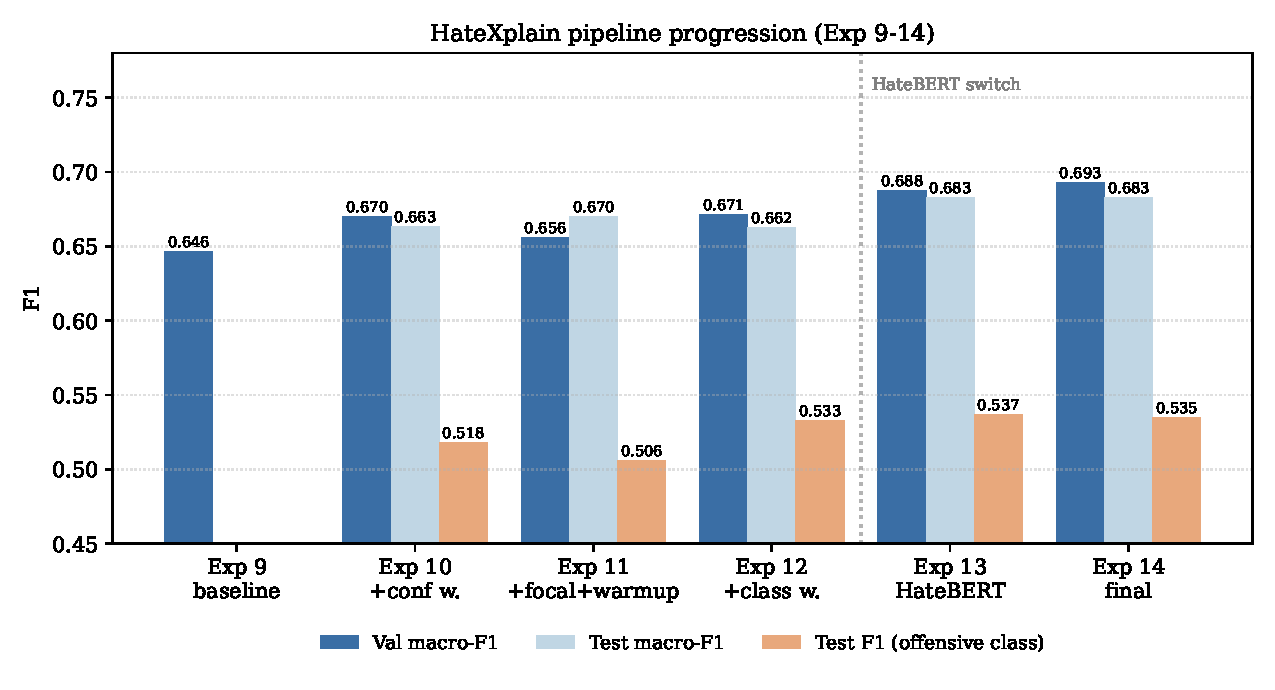
\includegraphics[width=\linewidth]{figures/fig1_hatexplain_progression.pdf}
\caption{HateXplain ablation: the HateBERT switch dominates ($+0.123$ val F1, beyond the dotted line). All other techniques combined add less.}
\label{fig:hatexplain}
\end{figure}

\subsection{HateXplain ablation (Fig.~\ref{fig:hatexplain})}
Going from roberta-base baseline (val F1 $0.647$) to confidence weighting ($+0.024$) to focal+warmup ($-0.014$, calibration $\uparrow$) to class weights ($+0.016$) brings val F1 to $0.672$. Swapping the backbone to HateBERT --- with everything else fixed --- adds $+0.121$ in a single step, validating H1. The final model (HateBERT + focal + warmup, no class weights) reaches val F1 $0.693$ and test F1 $0.683$. Residual errors are dominated by the symmetric offensive$\leftrightarrow$normal confusion ($149$ vs $150$ examples), matching the 33\% annotator disagreement on the \emph{offensive} class~\cite{hatexplain}: this is an annotation, not a modelling, boundary.

\subsection{Target-group bias (Fig.~\ref{fig:bias})}
On the final model we measure a $0.22$ macro-F1 gap between the worst group (Asian, $0.467$, $n{=}53$) and the best (Other, $0.690$, $n{=}244$). The six worst-performing groups are all racial/ethnic minorities. Diagnosis: these groups appear predominantly in hateful contexts in training (Jewish 68\% hate, African 60\%, Arab 59\%), so the model learns a ``group mention $\Rightarrow$ hate'' shortcut~\cite{davidson,sap}.

% ---- Figure 2 : Per-group bias ----
\begin{figure}[t]
\centering
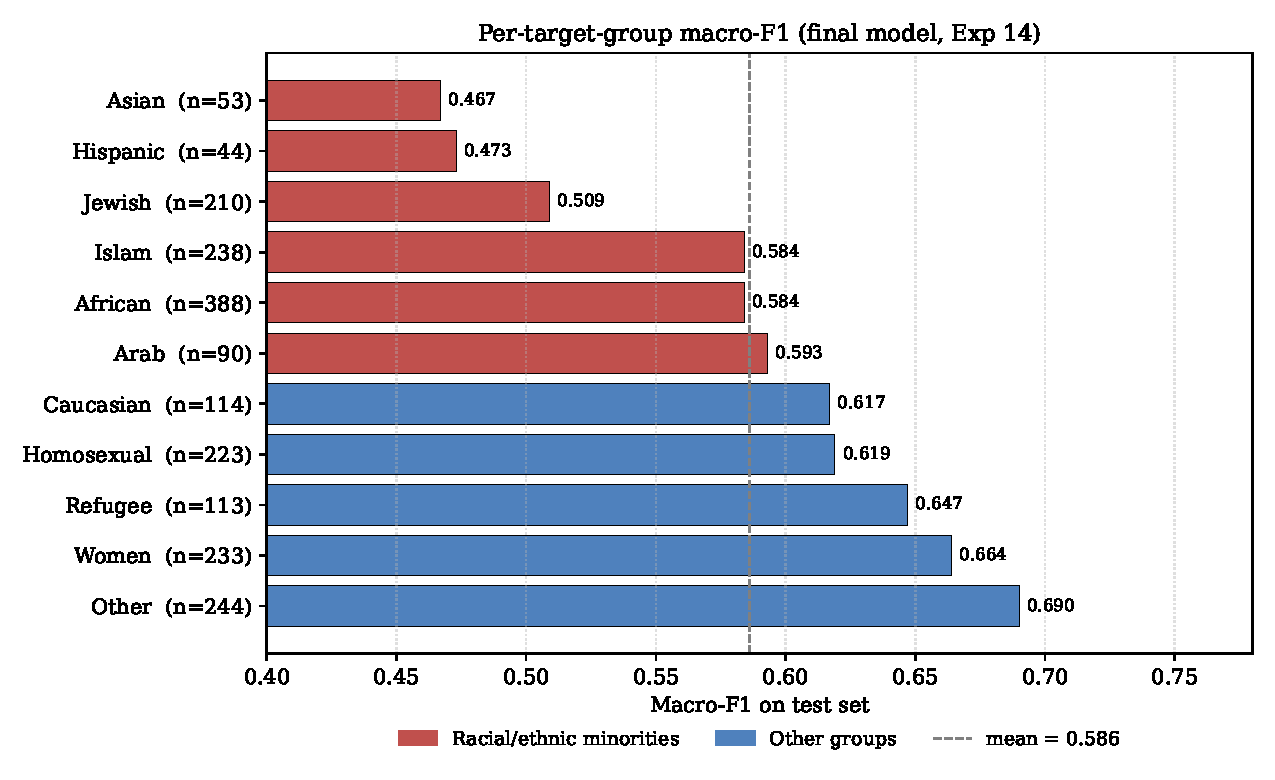
\includegraphics[width=\linewidth]{figures/fig2_bias_per_group.pdf}
\caption{Per-target-group macro-F1 of the final HateXplain model. The six worst groups are all racial/ethnic minorities, indicating a learned shortcut from group mention to hate label.}
\label{fig:bias}
\end{figure}

\textbf{Mitigation results.}
Test macro-F1 / bias gap:
baseline $0.683$ / $\mathbf{0.223}$;
group-aware weighting $0.658$ / $0.264$;
CF-augment (hate+off only) $0.666$ / $0.306$;
CF-augment (balanced) $0.640$ / $0.265$. \emph{Both interventions worsen the gap and overall F1.} We attribute this to (i) HateBERT's RAL-E pre-training already embedding group-hate co-occurrences at every layer, so ${\sim}10^3$ synthetic substitutions cannot compete with millions of pre-training tokens (validating H3), and (ii) training-set scarcity for the smallest groups (Asian $n{\approx}50$, Hispanic $n{\approx}44$): re-weighting cannot create signal where there is no data, consistent with~\cite{davidson}.

\subsection{Multimodal architecture ablation on HarMeme (Fig.~\ref{fig:harmeme})}
Frozen: AUC $0.877$, F1 $0.751$. Defrost: AUC $\mathbf{0.910}$, F1 $\mathbf{0.804}$ (best). Cross-attention + defrost: AUC $0.883$, F1 $0.691$ (val-tuned $0.772$). Uniform ensemble: AUC $0.899$ (worse than defrost alone). Ensemble + TTA (flip $+$ 5-crops): AUC $0.891$ (further degraded). Defrost wins because $3013$ examples are sufficient to refine the last two encoder layers but insufficient to train $28$\,M random cross-attention parameters from scratch (validating H2). TTA hurts because the harmful signal is the burned-in text overlay, which flip-and-crop transforms violate by construction.

% ---- Figure 3 : HarMeme architectures ----
\begin{figure}[t]
\centering
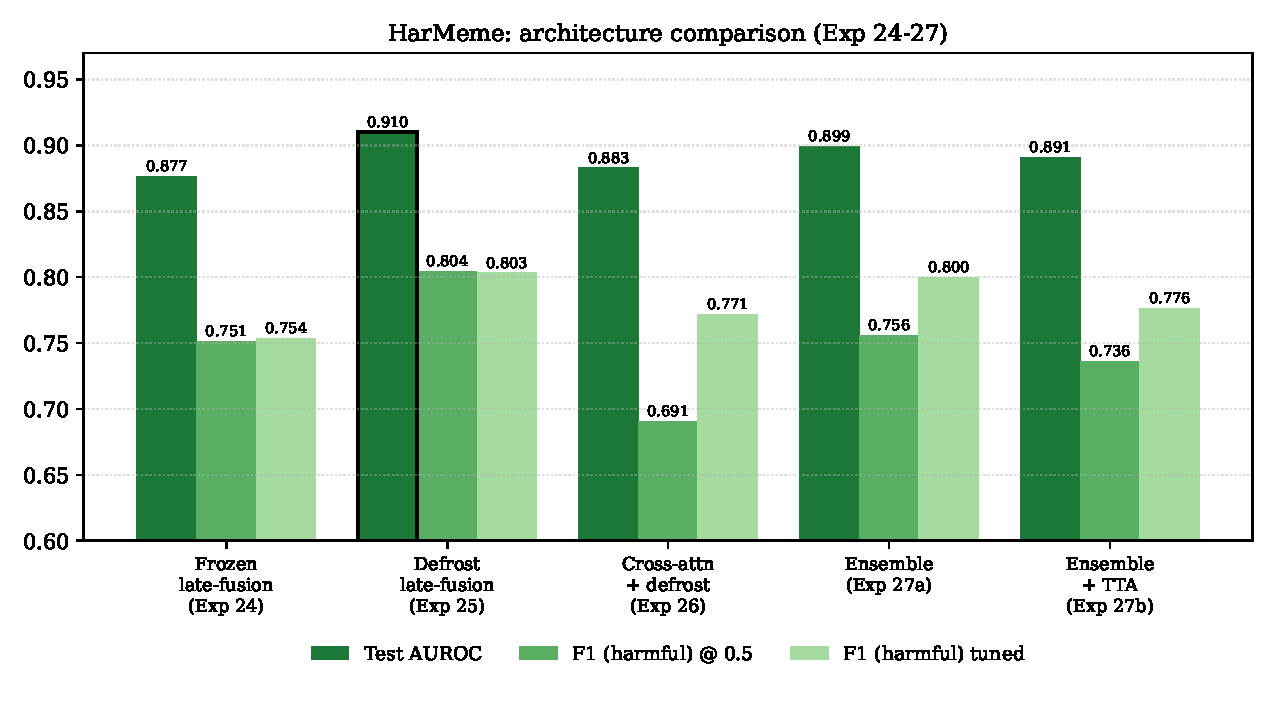
\includegraphics[width=\linewidth]{figures/fig4_harmeme_archs.pdf}
\caption{HarMeme: defrosting the last 2 layers (Exp~25) clearly beats both frozen and cross-attention fusion. Ensembling pulls performance back toward the weaker members; TTA further degrades F1.}
\label{fig:harmeme}
\end{figure}

\subsection{Dataset-loading bug --- methodological lesson}
During development we used the HuggingFace snapshot \texttt{limjiayi/hateful\_memes\_expanded}, which ships JSONL metadata only --- the image files do not exist on disk. Our \texttt{HatefulMemesDataset} silently returned a uniform-grey RGB image on \texttt{FileNotFoundError}. \textbf{All eight prior multimodal experiments were therefore text-only models in a multimodal wrapper.} We detected this by checking whether \texttt{torch.flip(pixel\_values, dims=[3])} changes the output logits --- it did not. We fixed the loader to fail loudly (\texttt{strict\_images: true}) and pivoted to HarMeme, which ships real images.

\subsection{Limitations}
\textbf{(L1)} Single-seed evaluation: variance was not estimated; literature suggests $\pm 0.003$--$0.01$ macro-F1 across seeds for similar setups. \textbf{(L2)} HarMeme test set is small ($354$ examples); AUROC differences below $0.01$ are not statistically meaningful. \textbf{(L3)} Hateful Memes was not reproducible locally (DrivenData archived the competition; HF copies are metadata-only). HarMeme is on a different topic (COVID) and smaller than Hateful Memes, so multimodal numbers are not comparable to the literature reporting on Hateful Memes. \textbf{(L4)} We did not implement adversarial debiasing~\cite{zhang} or LLM-generative augmentation, both of which may succeed where our naive interventions failed.

% =============================================================
\section{Conclusion}
% =============================================================

Domain-adapted pre-training (HateBERT) dominates architectural and loss tricks on HateXplain. On a small multimodal benchmark (HarMeme), partial defrost of the last two encoder layers beats both fully frozen encoders and cross-attention fusion. Two simple bias-mitigation strategies failed in a reproducible way, mapping the practical limits of surface-level corrections. Beyond raw metrics, our most transferable finding is methodological: a silent data-loader fallback almost cost us our entire multimodal study, and a two-line invariance check would have caught it instantly.

\vspace{-0.3em}
\begin{thebibliography}{99}\small
\setlength{\itemsep}{0pt}\setlength{\parsep}{0pt}

\bibitem{hatexplain} B.~Mathew \emph{et al.}, ``HateXplain: A benchmark dataset for explainable hate speech detection,'' in \emph{Proc.\ AAAI}, 2021.

\bibitem{hatebert} T.~Caselli \emph{et al.}, ``HateBERT: Retraining BERT for abusive language detection in English,'' in \emph{Proc.\ WOAH}, 2021.

\bibitem{clip} A.~Radford \emph{et al.}, ``Learning transferable visual models from natural language supervision,'' in \emph{Proc.\ ICML}, 2021.

\bibitem{focal} T.-Y.~Lin \emph{et al.}, ``Focal loss for dense object detection,'' in \emph{Proc.\ ICCV}, 2017.

\bibitem{kiela} D.~Kiela \emph{et al.}, ``The hateful memes challenge: Detecting hate speech in multimodal memes,'' in \emph{Proc.\ NeurIPS}, 2020.

\bibitem{harmeme} S.~Pramanick \emph{et al.}, ``Detecting harmful memes and their targets,'' in \emph{Findings of ACL}, 2021.

\bibitem{davidson} T.~Davidson \emph{et al.}, ``Racial bias in hate speech and abusive language detection datasets,'' in \emph{Proc.\ ACL Workshop on Abusive Language Online}, 2019.

\bibitem{sap} M.~Sap \emph{et al.}, ``The risk of racial bias in hate speech detection,'' in \emph{Proc.\ ACL}, 2019.

\bibitem{liang} P.~P.~Liang \emph{et al.}, ``Towards debiasing sentence representations,'' in \emph{Proc.\ ACL}, 2020.

\bibitem{zhang} B.~H.~Zhang \emph{et al.}, ``Mitigating unwanted biases with adversarial learning,'' in \emph{Proc.\ AIES}, 2018.

\bibitem{howard-ulmfit} J.~Howard and S.~Ruder, ``Universal language model fine-tuning for text classification,'' in \emph{Proc.\ ACL}, 2018.

\end{thebibliography}

\end{document}
{document}
